\documentclass[msc,m,palatino,oneside,12pt]{softlang}

% Use one of the following terms and replace msc as argument in documentclass:
% Master of Science thesis: msc
% Bachelor of Science thesis: bsc
% Projektpraktikum: pp
% Diplomarbeit: diplom
% Proseminar: prosem
% Seminararbeit: sem
% Skript: scr
% Studienarbeit: sa

% Use m(Männlich) or w(Weiblich) as argument in documentclass
% 12pt is the size of the text
% oneside is for normal text layout, the text is centered
% twoside prints the text assymmetric
% palatino is tzhe font of the letters


% BibLatex for Bibliography
% For Citation- and Bibliographystyles refer to the biblatex documentation
% Standard is numeric both
\usepackage{biblatex}
\addbibresource{sources.bib}

% This are optional packages, to use them remove the %:
\usepackage{booktabs} %for optimicing tabulars
%\usepackage{bibgerm} % for german BibTex styles
\usepackage{wrapfig}% for wrapping text arount tables and figures
\usepackage{multicol} % for Intermix single and multiple columns
\usepackage{enumitem} % for more options in the enumerate environment
\usepackage{subcaption} % for subfigures
\usepackage[font=footnotesize,labelfont=bf,labelsep=space]{caption} % for more formatting captions
\usepackage{tikz} % for PGF/TikZ support
\usepackage{tabularx} % for advanced tables
\usepackage{listings} % for code listings
\usepackage{multirow} % for columns spanning multiple rows in tables

% Settings for the listings package, for additional settings refer to the listings package documentation
\lstset{
	breaklines=true, % Autozeilenumbruch bei langen Codezeilen
	breakatwhitespace=true, % Erlaube Zeilenumbruch nur bei Whitespace
	numbers = left, % Zeilennummern
	tabsize = 3, % Tabulatorabstand
	frame = single % Rahmen um Sourcecode listings
	}

% Bestimmt die Tiefe in der die Kapitel nummeriert werden
\setcounter{secnumdepth}{3}

% Bestimmt die Tiefe in der die Kapitel im Inhaltsverzeichnis erscheinen
\setcounter{tocdepth}{2}

% Set headheight to 15 pt to avoid fancyhdr warning
\setlength{\headheight}{15pt}

\author{<Name des/r Studierenden>}
\title{<Titel der Arbeit>}
\studiengang{<Studiengang>}

\makeatletter
%% Set the metadata for the PDF document and the colors of the internal links.
%% All colors are set to black in order to avoid unnecessary colorfulness.
\hypersetup{
	pdftitle    = {\@title},
	pdfauthor   = {\@author},
	pdfkeywords = {keyword1,keyword2,...,keywordn}, % Add some key words if you want.
	colorlinks  = true,
	unicode     = true,
	linkcolor   = black,
	citecolor   = black,
	filecolor   = black,
	urlcolor    = blue,
}
\makeatother


\erstgutachter{Prof.\ Dr.\ Ralf Lämmel}
\erstgutachterInfo{Institut für Informatik}

\zweitgutachter{Msc. Marcel Heinz}
\zweitgutachterInfo{Institut für Informatik}

% \drittgutachter{Hakan Aksu}
% \drittgutachterInfo{Institut für Informatik}


%% Beware of widows and orphans.
\clubpenalty         = 10000
\widowpenalty        = 10000
\displaywidowpenalty = 10000




%%%%%%%%%%%%%%%%%%%%%%%%%%%%%%%%%%%%%%%%%%%%%%%%%%%%%%%%%%%%

\begin{document}
\pagenumbering{Alph}
\pagestyle{empty}

\maketitle
\cleardoublepage

\subsection*{Zusammenfassung}

Deutsches Abstract (erforderlich laut Prüfungsordnung).


\subsection*{Abstract}

English abstract.
 % Einfügen des Abstracts
\cleardoublepage

%\pagestyle{headings}
\pagestyle{fancy}

\fancyfoot{}% Unten nichts
%\fancyhead[RE]{\itshape\leftmark}  % Rechts auf geraden Seiten=innen
%\fancyhead[RO]{\itshape\rightmark} % Links auf ungeraden Seiten=außen
\fancyhead[R]{\thepage}        % nur rechts

\pagenumbering{roman}
\tableofcontents

\cleardoublepage

\listoffigures   % fuer ein eventuelles Abbildungsverzeichnis
\cleardoublepage

% \listoftables % Für ein Tabellenverzeichnis
% \cleardoublepage

% \lstlistoflistings % Für ein Verzeichnis der Listings
% \cleardoublepage

\pagenumbering{arabic}


% Hier kommt jetzt der eigentliche Text der Arbeit
% Diese Datei dient nur als Include-File für die groben Gliederungspunkte

\chapter{Einleitung}

\section{Zitate einfügen}\label{sec:citation}
\cite{lammel2008google}
\cite{lammel2015software}

\section{Bilder einfügen}
\begin{figure}[h]
	\centering
	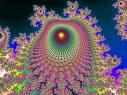
\includegraphics[width=0.60\textwidth]{images/image.jpg}
	\caption[Text im Abbildungsverzeichnis]{Text unter Abbildung}
	\label{fig:image}
\end{figure}

\section{Referenzieren}
Referenz zu einem Kapitel: \ref{sec:citation}

Referenz zu einem Bild: \ref{fig:image}

\section{Tabellen einfügen}

Schönere Tabellen als die \LaTeX-Standardtabellen lassen sich mit dem Paket {\tt booktabs} erzeugen. Dieses Paket ist in diesem Framework schon eingebunden. Ein Beispiel für eine solche schöne Tabelle zeigt Tabelle~\ref{tab:myVeryFirstTable}.

\begin{table}
	\center
	\begin{tabular}{l l l l}
		\toprule
		\bfseries{Spaltenüberschrift~1} & \bfseries{Spaltenüberschrift~2} & \bfseries{Spaltenüberschrift~3} \\
		\midrule
		Zelle~$(1,1)$                   & Zelle~$(1,2)$                   & Zelle~$(1,3)$                   \\
		Zelle~$(2,1)$                   & Zelle~$(2,2)$                   & Zelle~$(2,3)$                   \\
		Zelle~$(3,1)$                   & Zelle~$(3,2)$                   & Zelle~$(3,3)$                   \\
		\bottomrule
	\end{tabular}
	\caption
  	[Kurzer Text im Tabellenverzeichnis]
  	{Diese Tabelle kann auch etwas umfangreicher beschrieben werden. In diesem Fall bietet es sich an, für das Tabellenverzeichnis einen kürzeren Text zu definieren.}
  \label{tab:myVeryFirstTable}
\end{table}

Soll eine Zelle einer Tabelle über zwei oder mehr Zeilen laufen, bietet sich die Verwendung des Pakets {\tt multirow} an. Ein Beispiel für eine solche Tabelle zeigt Tabelle~\ref{tab:myMultiRowTable}.

\begin{table}
	\center
	\begin{tabular}{l l l l}
		\toprule
		\bfseries{Spalte~1} & \bfseries{Spalte~2} & \bfseries{Spalte~3} & \bfseries{Spalte~4} \\
		\midrule
		\multirow{2}{*}{Zelle~$\alpha$} & Zelle~$(1,2)$ & Zelle~$(1,3)$ & Zelle~$(1,4)$  \\
	                                  & Zelle~$(2,2)$ & Zelle~$(2,3)$ & Zelle~$(2,4)$  \\
		\midrule
		\multirow{2}{*}{Zelle~$\beta$}  & Zelle~$(3,2)$ & Zelle~$(3,3)$ & Zelle~$(3,4)$  \\
	                                  & Zelle~$(4,2)$ & Zelle~$(4,3)$ & Zelle~$(4,4)$  \\
		\bottomrule
	\end{tabular}
	\caption
  	{Tabelle mit {\tt multirow}s.}
  \label{tab:myMultiRowTable}
\end{table}

\section{Code einfügen}
Sourcecode lässt sich gut über die Umgebung lstlisting einfügen, man kann entweder die Sprache über lstset oder
direkt über die Umgebung setzen. Einige Optionen wie Rahmen um den Code und Zeilennummern wurden standardmäßig in der ausarbeitung.tex gesetzt. 

\lstset{language=Haskell}
\begin{lstlisting}[language=Haskell,caption=Lineare Suche]
search::Eq a => [a] -> a -> Bool
search [] _ = False
search (x:xs) a = 
	if x /= a
	then search xs a
	else True 
\end{lstlisting}

Mit lstinputlisting kann eine Sourcecode File importiert werden, über firstline und lastline kann kontrolliert werden welche Zeilen gedruckt werden.
\lstinputlisting[firstline=5,lastline=7,caption=Quicksort]{code/quicksort.hs}

\subsection{Unterabschnitt}

Lorem ipsum dolor sit amet, consetetur sadipscing elitr, sed diam nonumy eirmod tempor invidunt ut labore et dolore magna aliquyam erat, sed diam voluptua. At vero eos et accusam et justo duo dolores et ea rebum. Stet clita kasd gubergren, no sea takimata sanctus est Lorem ipsum dolor sit amet. Lorem ipsum dolor sit amet, consetetur sadipscing elitr, sed diam nonumy eirmod tempor invidunt ut labore et dolore magna aliquyam erat, sed diam voluptua. At vero eos et accusam et justo duo dolores et ea rebum. Stet clita kasd gubergren, no sea takimata sanctus est Lorem ipsum dolor sit amet.

\subsubsection{Unterunterabschnitt}

Generell sollte eine vierte Überschriftenebene wie diese hier vermieden werden.

Lorem ipsum dolor sit amet, consetetur sadipscing elitr, sed diam nonumy eirmod tempor invidunt ut labore et dolore magna aliquyam erat, sed diam voluptua. At vero eos et accusam et justo duo dolores et ea rebum. Stet clita kasd gubergren, no sea takimata sanctus est Lorem ipsum dolor sit amet. Lorem ipsum dolor sit amet, consetetur sadipscing elitr, sed diam nonumy eirmod tempor invidunt ut labore et dolore magna aliquyam erat, sed diam voluptua. At vero eos et accusam et justo duo dolores et ea rebum. Stet clita kasd gubergren, no sea takimata sanctus est Lorem ipsum dolor sit amet.

\chapter{Grundlagen}

Nach jeder Überschrift sollte ein Einleitungssatz stehen.
\section{Abschnitt}

Lorem ipsum dolor sit amet, consetetur sadipscing elitr, sed diam nonumy eirmod tempor invidunt ut labore et dolore magna aliquyam erat, sed diam voluptua. At vero eos et accusam et justo duo dolores et ea rebum. Stet clita kasd gubergren, no sea takimata sanctus est Lorem ipsum dolor sit amet. Lorem ipsum dolor sit amet, consetetur sadipscing elitr, sed diam nonumy eirmod tempor invidunt ut labore et dolore magna aliquyam erat, sed diam voluptua. At vero eos et accusam et justo duo dolores et ea rebum. Stet clita kasd gubergren, no sea takimata sanctus est Lorem ipsum dolor sit amet.

\subsection{Untersabschnitt}

Lorem ipsum dolor sit amet, consetetur sadipscing elitr, sed diam nonumy eirmod tempor invidunt ut labore et dolore magna aliquyam erat, sed diam voluptua. At vero eos et accusam et justo duo dolores et ea rebum. Stet clita kasd gubergren, no sea takimata sanctus est Lorem ipsum dolor sit amet. Lorem ipsum dolor sit amet, consetetur sadipscing elitr, sed diam nonumy eirmod tempor invidunt ut labore et dolore magna aliquyam erat, sed diam voluptua. At vero eos et accusam et justo duo dolores et ea rebum. Stet clita kasd gubergren, no sea takimata sanctus est Lorem ipsum dolor sit amet.
\chapter{Fazit}

Nach jeder Überschrift sollte ein Einleitungssatz stehen.

\section{Abschnitt}

Lorem ipsum dolor sit amet, consetetur sadipscing elitr, sed diam nonumy eirmod tempor invidunt ut labore et dolore magna aliquyam erat, sed diam voluptua. At vero eos et accusam et justo duo dolores et ea rebum. Stet clita kasd gubergren, no sea takimata sanctus est Lorem ipsum dolor sit amet. Lorem ipsum dolor sit amet, consetetur sadipscing elitr, sed diam nonumy eirmod tempor invidunt ut labore et dolore magna aliquyam erat, sed diam voluptua. At vero eos et accusam et justo duo dolores et ea rebum. Stet clita kasd gubergren, no sea takimata sanctus est Lorem ipsum dolor sit amet.

\subsection{Untersabschnitt}

Lorem ipsum dolor sit amet, consetetur sadipscing elitr, sed diam nonumy eirmod tempor invidunt ut labore et dolore magna aliquyam erat, sed diam voluptua. At vero eos et accusam et justo duo dolores et ea rebum. Stet clita kasd gubergren, no sea takimata sanctus est Lorem ipsum dolor sit amet. Lorem ipsum dolor sit amet, consetetur sadipscing elitr, sed diam nonumy eirmod tempor invidunt ut labore et dolore magna aliquyam erat, sed diam voluptua. At vero eos et accusam et justo duo dolores et ea rebum. Stet clita kasd gubergren, no sea takimata sanctus est Lorem ipsum dolor sit amet.

% Fuer einen Anhang die nachfolgenden Zeilen einkommentieren.
% \appendix
% \chapter{Not the Organ}\label{ch:not-the-organ}

Again, if you don't need your appendix, just delete this file.


\cleardoublepage
%\bibliographystyle{alphadin}
\printbibliography
\end{document}

